\begin{center}
\large \textbf{Písemná práce:} výroky a množiny \textbf{(varianta A)}

\normalsize
\makebox[8cm]{\textsc{Jméno:}\enspace\hrulefill}\qquad
\makebox[3cm]{\textsc{Třída:}\enspace\hrulefill}\qquad
\makebox[4cm]{\textsc{Datum:}\enspace\hrulefill}
\end{center}
\begin{table}[h]
\centering

\todo{Přepočítat body}\\
\begin{tabular}{c|c|c|c|c|c}
    \textbf{Body}   & $10-9$ & $8-7$ & $6-5$ & $4-3$ & $2-0$ \\ \hline
    \textbf{Známka} & $1$     & $2$   & $3 $  & $4$   & $5$
\end{tabular}
\end{table}

% \printanswers


\begin{questions}
    \question
        Určete, zda se jedná o výroky:
        \begin{parts}
            \part[\half]\TFQuestion{T}{Číslo 12 je prvočíslo.}
            \part[\half]\TFQuestion{F}{Přines mi prosím kapesník.}
            \part[\half]\TFQuestion{T}{$\forall x \in \mathbb{Z}: x + 3 > 0$}
        \end{parts}
    
    \question
        Určete negace kvantifikovaných výroků:   
        \begin{parts}
            \part[1]Alespoň jeden cestující nevystoupil.
            \begin{solutionordottedlines}[1cm]
                Všichni cestující vystoupili.
            \end{solutionordottedlines}

            \part[1]Právě jedna moje učebnice je těžká.
            \begin{solutionordottedlines}[1cm]
                Žádná moje učebnice nebo alespoň dvě moje učebnice jsou těžké.
            \end{solutionordottedlines}
        \end{parts}

    \question
        Negujte následující výroky:
        \begin{parts}
            \part[2]Každé přirozené číslo, které je dělitelné dvaceti, je dělitelné čtyřmi. 
            \begin{solutionordottedlines}[2cm]
                Existuje alespoň jedno přirozené číslo, které je dělitelné dvaceti a není dělitelné čtyřmi.
            \end{solutionordottedlines}

            \part[2]Do kina půjdu s Terkou nebo s Eliškou 
            \begin{solutionordottedlines}[1cm]
                Do kina nepůjdu s Terkou a nepůjdu ani s Eliškou.
            \end{solutionordottedlines}
        \end{parts}

    \question
        Kvantifikované výroky zapsané symbolicky vyjádřete slovy a rozhodněte o jejich pravdivosti:
        \begin{parts}
            \part[1 \half] $\forall x \in \mathbb{Z}: \sqrt{x^2} = |x|$
            \begin{solutionordottedlines}[2cm]
                Výrok je pravdivý.\\
                Druhá odmocnina z druhé mocniny libovolného reálného čísla je rovna jeho absolutní hodnotě. 
            \end{solutionordottedlines}

            \part[1 \half] $\exists x \in \mathbb{R} \forall y \in \mathbb{R}: x \cdot y = y$
            \begin{solutionordottedlines}[2cm]
                Výrok je pravdivý.\\
                Existuje takové reálné číslo $x$, že pro všechna reálná čísla $y$ platí $x \cdot y = y$  
            \end{solutionordottedlines}
        \end{parts}

    \question[1]
        Vypište všechny prvky následující množiny:
        $$ M = \{\xi \in \mathbb{Z}: -27 < \xi^3 \leq 8 \} $$
        \begin{solution}[2cm]
            $$M = \{ -2, -1, 0, 1, 2\}$$ 
        \end{solution}
    
    \question[3] 
        Mějme zadány intervaly $A = \langle 0, 18 \rangle$, $B = (13, 28) $ a $C = \langle 15, 17 \rangle$. Určete $((A \displaystyle \cap B) \setminus C)'$
        \begin{solution}[5cm]
            \begin{align*}
                A \displaystyle \cap B                  &= ( 13,18 \rangle\\
                (A \displaystyle \cap B) \setminus C    &= (13,15) \displaystyle \cup (17,18\rangle\\
                ((A \displaystyle \cap B) \setminus C)' &= (-\infty 13\rangle \displaystyle \cup  \langle 15,17\rangle \displaystyle \cup (18, \infty)
            \end{align*}
        \end{solution}

    \question[2]
        Ve třídě je 29 žáků, 19 z nich umí lyžovat, 12 jezdí na snowboardu, 5 jich nelyžuje a ani nejezdí na snowboardu. 
        Znázorněte pomocí Vennova diagramu a~určete, kolik žáků umí lyžovat i~jezdit na snowboardu.

        \begin{solution}[20cm]
            Označme si množinu všech žáků třídy jako $T$, $|T| = 29$. Žáky, kteří umí lyžovat označíme $L$, $|L| = 19$. 
            Snowboardisty označíme $S$, $|S| = 12$. Žáků, kteří neumí ani lyžovat ano na snowboardu je celkem $5$. Tedy 
                
                $$ |L \displaystyle \cup S| = 29 - 5 = 24 $$

            žáků umí buď lyžovat, nebo na snowboardu nebo obojí. Nyní, pokud sečteme žáky, co umí lyžovat a na snowboardu
            dostaneme 
                
                $$ 19 + 12 = 31\text{,} $$
            
            což odpovídá případu, kdy neexistuje ani jeden žák co umí na lyžích a snowboardu zároveň. Jelikož ale platí $31 > 24$,
            dostaneme informaci, že celkem 
                
                $$ 31 - 24 = \doubleunderline{7} $$
            
            žáků umí na lyžích a snowboardu zároveň.


            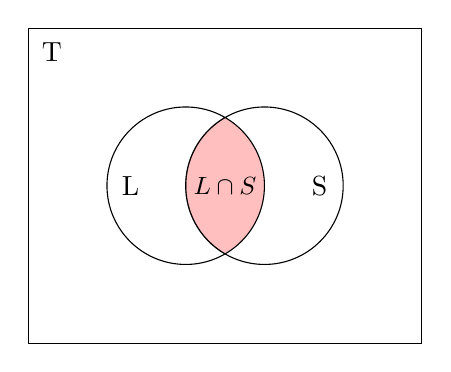
\begin{tikzpicture}
                \filldraw [fill=white] (-2.5,-2) rectangle (2.5,2);
                
                \scope % A \cap B
                \clip (-0.5,0) circle (1);
                \filldraw [fill=pink,draw opacity=0.5] (0.5,0) circle (1);
                \endscope

                % outline
                \draw (-0.5,0) circle (1)
                      (0.5,0) circle (1);

                \node (A) at (-2.2,1.7) {T};
                \node (B) at (1.2,0) {S};
                \node (B) at (-1.2,0) {L};
                \node (C) at (0,0) {\small$L \cap S$};
            \end{tikzpicture}
        \end{solution}        

\end{questions}

